% FID values for run11, run14 and run15 
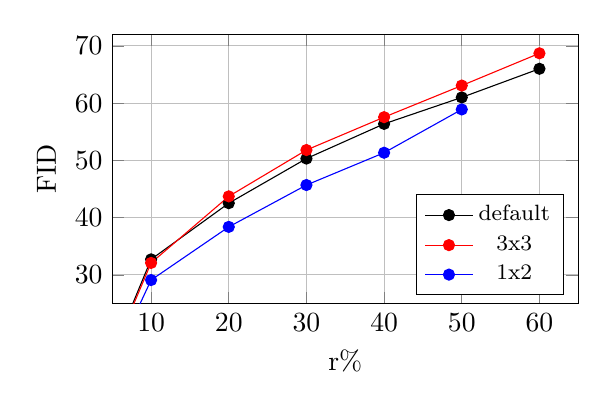
\begin{tikzpicture}
\begin{axis}[
    title={},
    height=5cm,
    width=7.5cm,
    xlabel={r\%},
    ylabel={FID},
    xmin=5, xmax=65,
    ymin=25, ymax=72,
    xtick={10,20,30,40,50,60},
    ytick={30,40,50,60,70},
    legend pos=south east,
    xmajorgrids=true,
    ymajorgrids=true,
    legend style={font=\footnotesize}
]

\addplot[
    color=black,
    mark=*
    ]
    coordinates {
    (0,0)(10,32.71)(20,42.52)(30,50.31)(40,56.37)(50,60.99)(60,65.99)
    };
    
\addplot[
    color=red,
    mark=*
    ]
    coordinates {
    (0,0)(10,32.09)(20,43.71)(30,51.80)(40,57.54)(50,63.06)(60,68.69)
    };

\addplot[
    color=blue,
    mark=*
    ]
    coordinates {
    (0,0)(10,29.10)(20,38.38)(30,45.69)(40,51.33)(50,58.89)
    };
    
\legend{default, 3x3, 1x2}
    
\end{axis}
\end{tikzpicture}